\documentclass{article}
\usepackage[utf8]{inputenc}

\usepackage[english]{babel}
\usepackage{array}
 
\usepackage{amsthm}
\usepackage{amssymb}
\usepackage{amsmath}
\usepackage{longtable}
\usepackage[utf8]{inputenc}

\usepackage{graphicx}
\usepackage{subcaption}

\usepackage{geometry}
 \geometry{
    a4paper,
    total={170mm,257mm},
    left=15mm,
    top=15mm,
}

\title{Counting Peg Solitaire Solutions}
\author{Niam Vaishnav}
\date{29th April 2020}

\begin{document}

\maketitle

\section{The Algorithm}

To count the number of ways of solving a peg solitaire problem, I used a depth first search approach. This means I would make as many moves as possible in a row before backtracking when the game has been completed or no new moves can be made.

I used this approach instead of a breadth first search as the stack used in DFS stays relatively short as opposed to the queue used in BFS, which for a grid with 5 rows ran out of memory almost immediately. This is because BFS adds every possible move to the queue at a given position which means it gets bery large very quickly. If the shortest path is required, then BFS would be better as the first result it finds would be the shortest.

Another important change I have made is I have ignored multi-move turns. This is because I don't think that doing 2 moves in one turn counts as a seperate solution, as it is just combining the moves in another solution. It also speeds up the program by a lot and keeps the stack empty.

The code was written in Scala, where I created a class for the board that contains the current position of the pieces. This was then used in a DFS algorithm. For convienience, the numbers have been altered so that the counting starts from 0, so the top position is marked by the number 0 and the bottom right is marked by $\frac{n(n-1)}{2} - 1$ when there are $n$ rows.

\section{The Results}

\subsection{4 Rows}

When there are 4 rows on the board, the starting empty squares can be split into three equivalence classses, where squares in the same class are related by symmetry:

\begin{align*}
    & E_1 = \{0, 6, 9\} \\
    & E_2 = \{1, 2, 3, 5, 7, 8\} \\
    & E_3 = \{4\}
\end{align*}

\begin{center}
    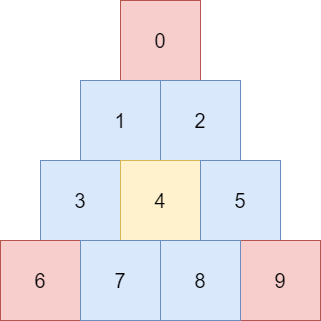
\includegraphics[width=0.3\linewidth]{"./Images/4EquivalenceClass.png"}
\end{center}

The classes $E_1$ and $E_3$ have no solutions. However, the 6 squares in $E_2$ are able to be solved, and each starting square has a unique empty square. The following table shows the number of ways we can get from a starting empty square to a ending filled square:

\begin{center}
\begin{tabular}{c | c c c c c c c c c c}
    & \multicolumn{10}{c}{End} \\
    Start  & 0 & 1 & 2 & 3 & 4 & 5 & 6 & 7 & 8 & 9 \\
    \hline
    0 & - & - & - & - & - & - & - & - & - & -\\
    1 & - & - & 14 & - & - & - & - & - & - & -\\
    2 & - & 14 & - & - & - & - & - & - & - & -\\
    3 & - & - & - & - & - & - & - & 14 & - & -\\
    4 & - & - & - & - & - & - & - & - & - & -\\
    5 & - & - & - & - & - & - & - & - & 14 & -\\
    6 & - & - & - & - & - & - & - & - & - & -\\
    7 & - & - & 14 & - & - & - & - & - & - & -\\
    8 & - & - & - & - & 14 & - & - & - & - & -\\
    9 & - & - & - & - & - & - & - & - & - & -
\end{tabular}
\end{center}

This can also be shown on a diagram:

\begin{center}
    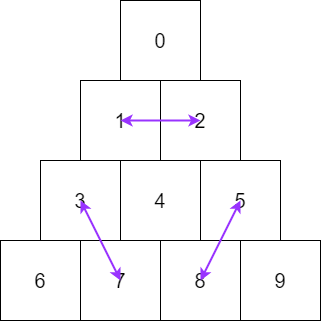
\includegraphics[width=0.3\linewidth]{"./Images/4Rows.png"}
\end{center}

I also calculated the shortest sequeunce of moves, where more than one jump can be made per move, using a BFS algorithm. There were two sequences of shortest length starting from square 1 being empty:

$$ 6-1 \  0-3 \  8-6-1 \  5-0-3-5 \ 9-2 $$
$$ 6-1 \  0-3 \  8-6-1 \  5-3-0-5 \ 9-2 $$

\subsection{5 Rows}

The results are much more interesting when there are 5 rows. In this case it is always possible to solve the problem no matter which square was taken out first. There are 4 equivalence classes in this case:

\begin{center}
\begin{align*}
    & E_1 = \{0, 10, 14\} \\
    & E_2 = \{1, 2, 6, 9, 11, 13\} \\
    & E_3 = \{3, 5, 12\} \\
    & E_4 = \{4, 7, 8\}
\end{align*}
\end{center}

\begin{center}
    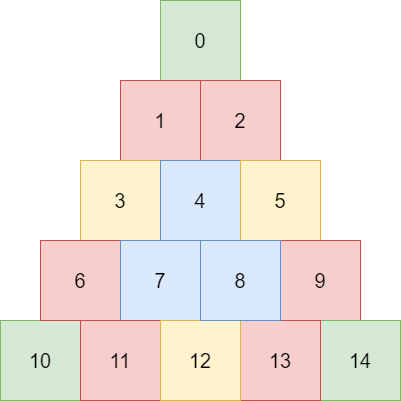
\includegraphics[width=0.3\linewidth]{"./Images/EquivalenceClasses.png"}
\end{center}

There are thousands of solutions for each starting square, and all of the squares apart from those in $E_4$ can reach more than one ending square:

\begin{center}
\begin{tabular}{c | c c c c c c c c c c c c c c c}
    & \multicolumn{15}{c}{End} \\
    Start  & 0 & 1 & 2 & 3 & 4 & 5 & 6 & 7 & 8 & 9 & 10 & 11 & 12 & 13 & 14\\
    \hline
    0 & 6816 & - & - & - & - & - & 3408 & - & - & 3408 & - & - & 16128 & - & -\\
    1 & - & 720 & - & - & - & 8064 & - & - & - & - & 3408 & - & - & 2688 & -\\
    2 & - & - & 720 & 8064 & - & - & - & - & - & - & - & 2688 & - & - & 3408\\
    3 & - & - & 8064 & 51452 & - & - & - & - & 1550 & - & - & 8064 & - & - & 16128\\
    4 & - & - & - & - & - & - & - & - & - & - & - & - & - & - & -\\
    5 & - & - & - & - & - & - & - & - & - & - & - & - & 1550 & - & -\\
    6 & - & 8064 & - & - & - & 15452 & - & 1550 & - & - & 16128 & - & - & 8064 & -\\
    7 & - & - & - & - & - & 1550 & - & - & - & - & - & - & - & - & -\\
    8 & - & - & - & 1550 & - & - & - & - & - & - & - & - & - & - & -\\
    9 & 3048 & - & - & - & - & - & 2688 & - & - & 720 & - & - & 8064 & - & -\\
    10 & - & 3048 & - & - & - & 16128 & - & - & - & - & 6816 & - & - & 3408 & -\\
    11 & - & - & 2688 & 8064 & - & - & - & - & - & - & - & 720 & - & - & 3408\\
    12 & - & 8064 & - & - & - & - & - & 1550 & - & - & 16128 & - & 51452 & 8064 & -\\
    13 & - & 2688 & - & - & - & 8064 & - & - & - & - & 3408 & - & - & 720 & -\\
    14 & - & - & 3048 & 16128 & - & - & - & - & - & - & - & 3048 & - & - & 6816
\end{tabular}
\end{center}
    
We can also put these on 4 diagrams:

\begin{center}
\begin{figure}[h]
    \begin{subfigure}[b]{1.7\linewidth}
        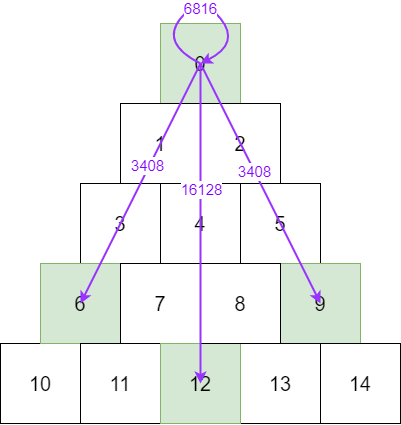
\includegraphics[width=0.25 \linewidth]{"./Images/0Class.png"}
        \hspace{1.5cm}
        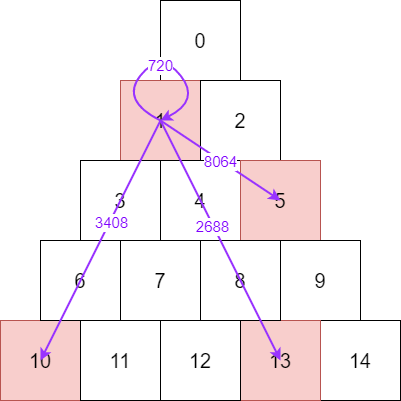
\includegraphics[width=0.25 \linewidth]{"./Images/1Class.png"}
    \end{subfigure}
    \par\bigskip
    \par\bigskip
    \begin{subfigure}[b]{1.7\linewidth}
        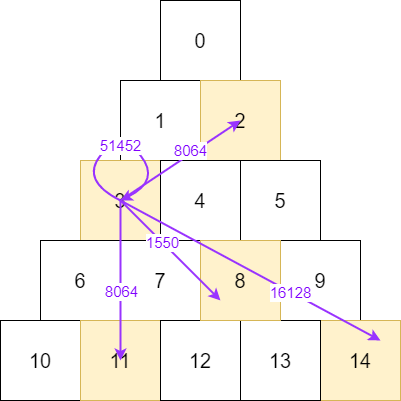
\includegraphics[width=0.25 \linewidth]{"./Images/3Class.png"}
        \hspace{1.5cm}
        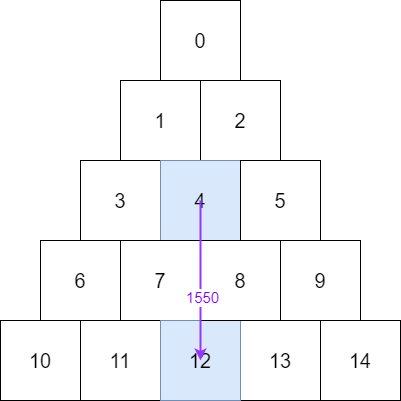
\includegraphics[width=0.25 \linewidth]{"./Images/4Class.png"}
    \end{subfigure}
\end{figure}
\end{center}

\end{document}